\section{Forecasting methods}
\subsection{Comparable simple benchmarks}
Let $\mathcal T_y$ contain only events in years strictly before test year $y$. For each held-out $(d,s,h)$ with $d$ in year $y$, we evaluate three rules without fitting a flexible predictor:
\begin{align}
\widehat Y^{(B)}_{dsh}&=B_{dsh}, \label{eq:baseordinary}\\
\widehat Y^{(E)}_{dsh}&=\operatorname{med}_{e\in\mathcal T_y}Y_{esh}, \label{eq:baseevent}\\
\widehat Y^{(B+E)}_{dsh}&=
\left[B_{dsh}+\operatorname{med}_{e\in\mathcal T_y}
  (Y_{esh}-B_{esh})\right]_+ . \label{eq:baseincrement}
\end{align}
The historical-event median is conditional on the same station and source hour; the excess rule transfers a prior-year median event increment to the current ordinary-day level. All predictions are clipped at zero. The first two rules are already nonnegative. No labels from the held-out year enter either median, and all three rules are scored on the same nine Beimen events as the frozen models. In contrast, $B_{dsh}$ can use earlier ordinary days from the target year because the archived feature was defined relative to each event date. Its contemporaneous release status remains unverified. These rules do not contain a forecasted event size, and the two event-analog rules are intentionally simple rather than tuned on the nine held-out events.

\subsection{Candidate features and common evaluation}
The model candidate set comprises station and source hour, their interaction, weekend status, day of year, a year trend, the ordinary-day level, and the first and second hours of overlap after a \emph{scheduled} finale, by station. Planned drone or weather variables were explored separately but are not part of the retained model. Standardized continuous columns are transformed using training-only moments; category references, imputation values and any rank-based column removal are also estimated inside the training fold. Strong correlation or a large variance-inflation factor warns about coefficient instability, but is neither a proof of causality nor an automatic instruction to remove a predictor from every model.

For test year $y\in\{2024,2025,2026\}$, fit on all preceding events and evaluate the complete Beimen events in year $y$. The training sets contain 12, 15 and 18 events, respectively. All six hours of an event stay together. Hyperparameter comparison within a year uses only earlier years; nevertheless, subsequent decisions made after examining these nine outer events introduce an additional model-selection risk. Define the primary forecast error and two peak-related summaries by
\begin{align}
\operatorname{MAE}&=\frac1n\sum_i|Y_i-\widehat Y_i|,&
\operatorname{RMSE}&=\sqrt{\frac1n\sum_i(Y_i-\widehat Y_i)^2},\label{eq:metrics}\\
\operatorname{Under}_{\mathcal D}
&=\sum_{i\in\mathcal D}a_i(Y_i-\widehat Y_i)_+,&
\operatorname{PeakAbs}
&=\frac1{|\mathcal E|}\sum_{e\in\mathcal E}
  |Y_{e,h_e^*}-\widehat Y_{e,h_e^*}|.\label{eq:peakmetrics}
\end{align}
Here $h_e^*=\arg\max_hY_{eh}$ is the \emph{observed} peak hour, used for retrospective scoring only. $\mathcal D$ and weights $a_i$ are determined from scheduled dispersal-hour overlap, normalized within events and then equally across events; if no scheduled overlap is known, the six event hours receive fallback weight. MAE and RMSE are per source hour. Positive underprediction and absolute peak error address different operational concerns.

\subsection{Linear models, GAM and tree boosting}
For treatment-coded and standardized design matrix $Z$ and training response $Y$, ordinary least squares minimizes $\|Y-\beta_0\mathbf1-Z\beta\|^2$. Ridge adds a squared penalty,
\begin{equation}
\min_{\beta_0,\beta}\,
\frac1n\|Y-\beta_0\mathbf1-Z\beta\|_2^2+
\lambda_R\|\beta\|_2^2,\qquad \lambda_R>0.
\label{eq:ridge}
\end{equation}
The Lasso replaces the penalty by $\lambda_L\|\beta\|_1$ \cite{lasso}. Ridge keeps correlated signals but shrinks them; Lasso can remove individual encoded columns and hence is more sensitive to scaling and penalization when predictors are related. These are conditional predictive associations, not treatment effects.

The Gaussian-identity GAM uses an additive linear predictor
\begin{equation}
g(X)=\beta_0+\sum_{j\in\mathcal S}f_j(X_j)+
\sum_{k\in\mathcal L}\theta_kX_k ,
\label{eq:gam}
\end{equation}
with cubic P-splines for approved smooth terms, second differences of spline coefficients penalized, and a positive all-coefficient $L_2$ term for stability \cite{gam,pspline}. The ordinary-day baseline is linear in this implementation. A partial-effect curve describes one component of this fitted additive function; its horizontal position is not a forecast error or a causal date effect.

XGBoost adds regularized trees $f_m$ sequentially \cite{xgb}. For a fixed candidate tree structure and a leaf with summed first and second derivatives $G_j,H_j$, the quadratic approximation has optimal leaf weight
\begin{equation}
w_j^*=-\frac{G_j}{H_j+\lambda_T},\qquad H_j+\lambda_T>0.
\label{eq:leaf}
\end{equation}
This is an optimum \emph{conditional on that leaf and approximation}; it proves neither a globally optimal tree ensemble nor superior external accuracy. Trees are included because threshold patterns and multiway station--hour--dispersal interactions need not be specified one at a time.

\subsection{Tuning, training weights and deployment choice}
The archived experiments inspected 25 Ridge penalties, 60 GAM smoothness/coefficient-penalty/basis combinations, and 180 prespecified XGBoost configurations (not the complete Cartesian product). Learning-rate/tree-count pairs and early stopping were also examined. After adding the ordinary-day feature, a previously fixed tree setting outperformed some retuned alternatives. The retained version uses the original year-specific tree settings and a training weight for Beimen scheduled dispersal:
\begin{equation}
\widetilde\omega_i=
1+3\,\ind\{s_i=\mathrm{Beimen}\}(o_{i,0\text{--}60}+o_{i,60\text{--}120}),
\qquad
\omega_i=\frac{\widetilde\omega_i}
{\overline{\widetilde\omega}_{\,e(i)}}.
\label{eq:weights}
\end{equation}
The denominator is the mean raw weight within the corresponding event. This fourfold maximum \emph{training-sample} emphasis is distinct from an asymmetric loss that charges twice as much for underprediction, and distinct from weights in a model fusion. The final model has depth 3, 250 trees and learning rate 0.10 in the 2024 fold; depth 4, 250 trees and learning rate 0.05 in the 2025 and 2026 folds. The retained settings use minimum child weight 1, $L_2$ leaf penalty 1, no $L_1$ leaf penalty and full row/column sampling; the final fit does not use early stopping.

Equal-weight and learned nonnegative combinations of Ridge, GAM and XGBoost were compared. Neither consistently surpassed the best tree in the archived comparison; the deployed demand input is therefore the single frozen weighted XGBoost, while linear models and GAM remain explanatory comparators. The existence of a minimum for a fusion-weight loss does not guarantee useful out-of-sample complementarity. Mathematical conditions are given in Appendix~\ref{sec:proofs}.

\section{Forecasting results}
\subsection{Simple baselines on identical held-out events}
Table~\ref{tab:benchmarks} reports the new standalone baselines and the archived forecast, evaluated using precisely the nine Beimen events and scorer in Section 4.2. The best simple rule is the ordinary-day level plus a prior-year station-hour median event excess. Its MAE of 1,233.76 is substantially smaller than the ordinary-day-only MAE of 2,027.50, demonstrating why the normal-day level is a weak \emph{sole} forecast for a special event. The frozen weighted XGBoost's MAE of 440.28 is lower by 793.48 entries per hour relative to that strongest simple rule. This is a retrospective comparison, not a claim of unbiased future improvement.
\begin{table}[htbp]\centering\small
\caption{Same-fold Beimen forecast comparison: nine events, 54 hours; counts are entries per hour.}
\label{tab:benchmarks}
\begin{tabular}{p{50mm}rrrr}\toprule
Method & MAE & RMSE & Peak absolute & Dispersal under\\\midrule
Ordinary-day profile & 2,027.50 & 3,281.47 & 6,277.41 & 4,628.28\\
Prior-year event median & 1,339.26 & 2,043.67 & 3,269.56 & 2,450.87\\
Ordinary + prior-year median excess & 1,233.76 & 1,940.49 & 3,196.39 & 2,320.54\\
\textbf{Frozen weighted XGBoost} & \textbf{440.28} & \textbf{690.91} & \textbf{747.14} & \textbf{483.61}\\\bottomrule
\end{tabular}
\end{table}
\begin{figure}[htbp]\centering
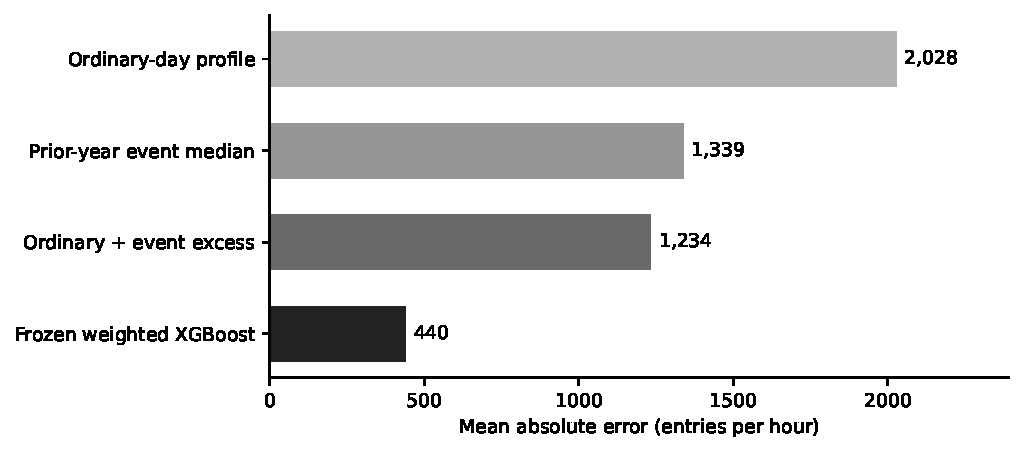
\includegraphics[width=.91\linewidth]{../../result/research_paper/figures/forecast_benchmark.pdf}
\caption{Hourly MAE for three prespecified simple rules and the archived weighted XGBoost on the same nine Beimen events. Lower is better.}
\label{fig:benchmark}
\end{figure}

\begin{table}[htbp]\centering\small
\caption{Event-level MAE for the strongest simple rule and frozen weighted XGBoost.}
\label{tab:eventmae}
\begin{tabular}{lrr@{\qquad}lrr}\toprule
Event & Excess rule & XGBoost & Event & Excess rule & XGBoost\\\midrule
2024-07-17 & 939.6 & 260.6 & 2025-08-20 & 782.4 & 220.3\\
2024-07-31 & 1,071.4 & 338.4 & 2025-08-30 & 1,861.2 & 326.8\\
2024-08-10 & 2,294.9 & 1,384.7 & 2026-07-25 & 1,312.5 & 375.5\\
2025-08-06 & 730.2 & 232.5 & 2026-08-05 & 487.3 & 275.5\\
2026-08-15 & 1,624.5 & 548.2 & & &\\\bottomrule
\end{tabular}
\end{table}
The XGBoost MAE is smaller on each of these nine events, but the worst event still has MAE 1,384.7. A paired resampling of \emph{events} yields a descriptive 2.5--97.5 percentile range of 566--1,035 entries per hour for the MAE advantage over the excess rule (20,000 fixed-seed resamples). It is not a confidence interval with guaranteed coverage for future events: only nine events are available, years may be dependent, and the frozen model itself was selected with prior inspection of this cohort. No statistical significance claim is based on this interval.

\subsection{Archived model-family comparisons and peak limitation}
On the same nine Beimen events, the archived Ridge, GAM, unweighted tree and weighted tree results are as in Table~\ref{tab:modelcompare}. This table answers a different question from Table~\ref{tab:benchmarks}: whether added model structure helped \emph{among the already constructed models}. The fourfold dispersal weight reduces MAE by about 7.1\% relative to the unweighted XGBoost, yet the scheduled dispersal-window underprediction increases from 405.96 to 483.61. The average-error improvement cannot be substituted for a claim that platform overload risk is resolved.
\begin{table}[htbp]\centering\small
\caption{Archived model-family results on the same nine-event Beimen cohort.}
\label{tab:modelcompare}
\begin{tabular}{lrrrr}\toprule
Model & MAE & RMSE & Peak absolute & Dispersal under\\\midrule
Ridge & 845.44 & 1,547.49 & 2,681.26 & 1,413.98\\
GAM & 830.71 & 1,315.75 & 2,305.11 & 1,132.68\\
XGBoost, unweighted & 473.91 & 766.90 & 749.02 & 405.96\\
XGBoost, dispersal weighted & 440.28 & 690.91 & 747.14 & 483.61\\\bottomrule
\end{tabular}
\end{table}

The teammate's separate linear sensitivity experiment retuned a different Ridge path and obtained original-scaling MAEs of 846.33 (OLS), 851.20 (retuned Ridge) and 848.52 (Lasso). Its Lasso improvement over that \emph{retuned} Ridge is only 2.68 entries per hour; the treatment of encoded columns and tuning differs from the frozen Ridge line above. The lower ex-post minimum along an inspected Lasso penalty path is not a selected prospective result. Thus Lasso remains a useful sparsity sensitivity analysis, but does not replace the retained forecast.

Figure~\ref{fig:peak} shows 10 August 2024. The observed Beimen maximum is about 11,101 entries, while the weighted tree predicts about 8,359 at that observed peak hour, an underprediction of about 2,742 (24.7\%). A station-hour ordinary-day profile is much lower. The event illustrates why a dispatch simulation should vary both demand error and remaining train capacity even if overall MAE is modest.
\begin{figure}[htbp]\centering
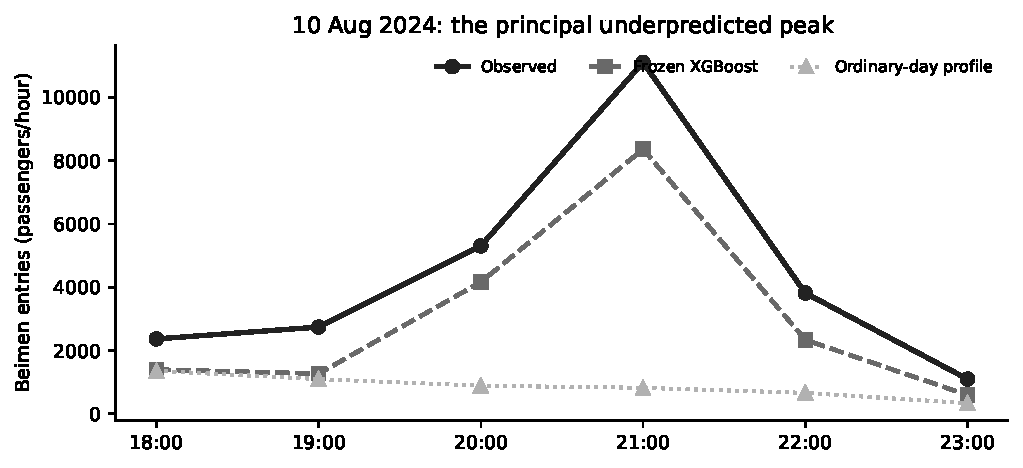
\includegraphics[width=.92\linewidth]{../../result/research_paper/figures/peak_profile.pdf}
\caption{Observed and predicted Beimen entries on 10 August 2024. The ordinary-day curve is a retrospective baseline, not an observed event-day forecast issued at the time.}
\label{fig:peak}
\end{figure}
\FloatBarrier
